%%%%%%%%%%%%%%%
%							DRAFT FLOOR PLAN
%%%%%%%%%%%%%%%

\subsection{Draft Floor Plan} \label{section:draft-floor-plan}

%New Paragraph
Before the schematics and floor plans for QUT's buildings were made available, an approximate small office area was modelled in AutoCAD with offices of 5\si{m^2} represented in Figure \ref{fig:RoughFloorplan}. The purpose of this simulation was to analyse approximate lighting loads for the environment. It was only used as a preliminary design approximation until more time was allocated to design.  

\begin{figure}[H]
\hfill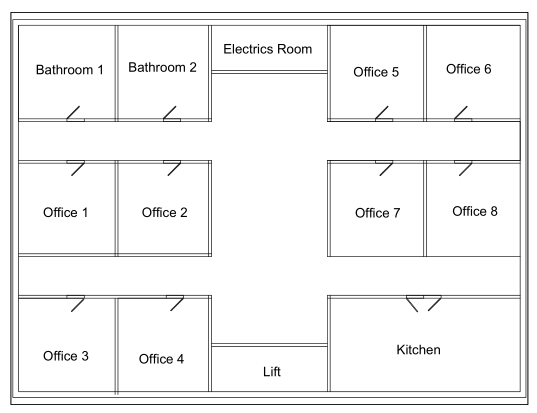
\includegraphics[width = 100mm]{images/Rough_Floorplan}\hspace*{\fill}
\caption{Initial Draft Floor Plan Design} 
\label{fig:RoughFloorplan}
\end{figure} 

\subsubsection{Draft Floor Plan Lighting Simulation}

%New Paragraph
After the initial room plans were created, the Australian Standards AS/NZS 1680.2.2 Interior and Workplace Lighting were consulted to produce a table of required lux values depending on room use. The standards is replicated and simplified below in Table \ref{table:LightingRequirements}.

\begin{table}[H]
\centering
\renewcommand{\arraystretch}{2}
\begin{tabular}{|l|c|}
\hline
\textbf{Area or Application} 	& \textbf{Lux Requirement} \\ \hline
Rarely Visited 					& 40 \\ \hline
Storage Rooms or Change Room 	& 80 \\ \hline
Machine Work or Waiting Room 	& 160 \\ \hline
Food Preparation Room 			& 240 \\ \hline
Technical Office Room 			& 320 \\ \hline
Visually Difficult Work 		& 500 \\ \hline
\end{tabular}
\caption{Lighting Requirements as per AS/NZS Standards \cite{StandardsAustralia2006_2}}
\label{table:LightingRequirements}
\end{table}

These two data points were used for the initial draft planning of designs. This is not an accurate representation of a building, it was a starting point to work from to beginning analysis load requirements. Once the more accurate schematics and plans are created, a stronger assessment can be created and feasibly power system construction plans created. To estimate load requirements for this smaller, draft area, the simple floor plan CAD file was imported into Dialux4.13. This is a lighting design software solution to model options and predict approximate load demands that the LVDC system will be required to power.  
\newline

%New Paragraph
Through personal experience in building services design, I had an approximate idea of what amounts of lighting would be required for a 5\,\si{m^2} room. I also knew that I would use LED down lights for simplicity and affordability. The difficult part is finding commercially available products that operate at a voltage level at either 48 V DC when the voltage drop over cabling is removed or at another level where an efficient DC to DC converter could be used. My goal was to have the average lux between 300\,\si{lux} to 400\,\si{lux}. This value was chosen as a technical office is an accurate assessment of most corporate buildings. As seen in Table \ref{table:draftFloorPlanDialuxOutputs} below, seven 20\,\si{W} LED down lights reaches this specification. The way this was completed was through multiple tested and rendering of designs. It can be a tedious process but photometric files (also known as IES files) are also imported into Dialux and can be placed throughout the 3D model. This 3D model is shown in Figure \ref{fig:DraftLighting3D}. To find the optimal solution, the simplest method is to remove and add lights of varying wattage and test the lux distribution. An example of the lux distribution is shown in Figure \ref{fig:DraftLightingLux}. Appendix \ref{appenddix:DraftFloorPlanLighting} shows the full report of the final working model.   

\begin{table}[!ht]
\centering
\renewcommand{\arraystretch}{1}
\begin{tabular}{|c|c|c|c|c|}
\hline
\multicolumn{1}{|l|}{\textbf{Down Light Wattage}} & \multicolumn{1}{l|}{\textbf{Quantity}} & \multicolumn{1}{l|}{\textbf{Max Lux}} & \multicolumn{1}{l|}{\textbf{Min Lux}} & \multicolumn{1}{l|}{\textbf{Average Lux}} \\ \hline
11 & 6 & 114 & 3.8 & 73 \\ \hline
11 & 10 & 180 & 7 & 114 \\ \hline
20 & 8 & 680 & 16 & 383 \\ \hline
20 & 7 & 677 & 12 & 344 \\ \hline
\end{tabular}
\caption{Dialux Outputs of Initial Draft Floor Plan}
\label{table:draftFloorPlanDialuxOutputs}
\end{table} 

\begin{figure}[H]
\hfill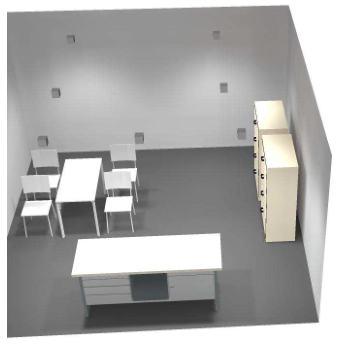
\includegraphics[width = 100mm]{images/lighting_draft_3D}\hspace*{\fill}
\caption{Initial Draft Floor Plan Lighting Test 3D Render} 
\label{fig:DraftLighting3D}
\end{figure} 

\begin{figure}[H]
\hfill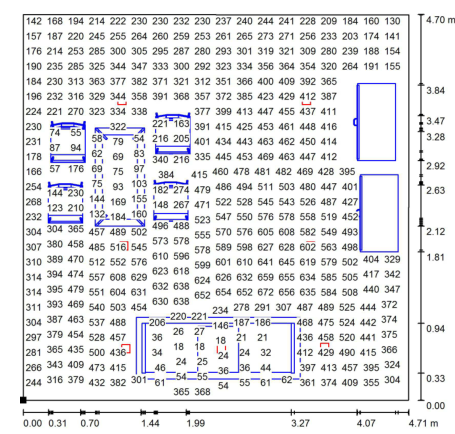
\includegraphics[width = 100mm]{images/lighting_draft_output}\hspace*{\fill}
\caption{Initial Draft Floor Plan Lighting Test Lux Output} 
\label{fig:DraftLightingLux}
\end{figure} 

%New Paragraph
Continuing from this example, the total lighting load of an office room would therefore be 140 W (20\,W * 7 lights). To approximate the total demand for the entire draft floor plan, there are bathrooms, kitchen and hallways that all require less light. If the offices' load is approximately 1.1 kW it can be expected that the total area lighting load would approach 1.8 kW. This is a good starting point and more accurate modelling can now be done with QUT's provided power data. 